\begin{frame}{Direct Detection mit Flavour-Mischung}
\vspace*{0.2cm}
\begin{columns}[c]
\begin{column}{.4\textwidth}
\begin{figure}[H]
	\resizebox{\textwidth}{!}{
		\begin{tikzpicture}
\tikzstyle{centerArrow}=[decoration={
markings,
mark=at position 0.5 with {\fill (2pt,0)--(-2pt,2.31pt)--(-2pt,-2.31pt)--cycle;}}]
\begin{scope}[xshift=3cm,yshift=-2cm]
\def\xmove{2}
\def\ymove{1.25}
\def\centerShift{2}
\def\centerSize{0.08cm}
\coordinate (tCenter1) at (0,0);
\coordinate[fill, circle,inner sep=\centerSize] (tCenter2) at (0,-\centerShift cm);
\node (upperLeft) at (-\xmove,\ymove) {$\chi$};
\node (upperRight) at (\xmove,\ymove) {$\chi$};
\node (lowerLeft) at (-\xmove,-\centerShift cm-\ymove cm) {$b_L,s_L$};
\node (lowerRight) at (\xmove,-\centerShift cm-\ymove cm) {$s_L,b_L$};
\node at (0.5,-\centerShift/2) {$Z'$};
\draw [centerArrow,postaction={decorate}]  (upperLeft) -- (tCenter1) ;
\draw [centerArrow,postaction={decorate}]  (tCenter1) -- (upperRight) ;
\draw [centerArrow,postaction={decorate}]  (lowerLeft) -- (tCenter2) ;
\draw [centerArrow,postaction={decorate}]  (tCenter2) -- (lowerRight) ;
\draw [decoration={snake, segment length=1.5mm, amplitude=0.5mm},decorate] (tCenter1) -- (tCenter2) ;
\end{scope}
\end{tikzpicture}
	}
	\caption{Tree-Wechselwirkung zur Streuung DM am Atomkern.}
\end{figure}
\end{column}
\begin{column}{.6\textwidth}
	\uncover<2->{Mögliche chirale Wechselwirkungen (Kopplungsstärke $C=q_\chi\frac{Y_{Qb}Y_{Qs}^*}{2m_Q^2}$):}
	\begin{align*}
		\only<2->{&Q_{2sb} = (\bar{\chi}\gamma_\mu\chi)(\bar{Q}_L^2\gamma^\mu Q_L^3)} \\
		\only<2->{&Q_{2bs} = (\bar{\chi}\gamma_\mu\chi)(\bar{Q}_L^3\gamma^\mu Q_L^2)}
	\end{align*}
	\uncover<3->{Nicht-chirale Wechselwirkungen:}
	\begin{align*}
		\only<3->{+&\text{Re}(V_{cd}^*V_{td}C)&&(\bar{\chi}\gamma_\mu\chi)(\bar{d}\gamma^\mu d)} \\
%%%%%%%%%%%%%%%%%%%%%%%%%%%%%%%%%%%%
		\only<3>{+&\text{Re}(V_{cs}^*V_{ts}C)&&(\bar{\chi}\gamma_\mu\chi)(\bar{s}\gamma^\mu s)}
		\only<4->{\textcolor{black!40}{+}&\textcolor{black!40}{\text{Re}(V_{cs}^*V_{ts}C)}&&\textcolor{black!40}{(\bar{\chi}\gamma_\mu\chi)(\bar{s}\gamma^\mu s)}} \\
%%%%%%%%%%%%%%%%%%%%%%%%%%%%%%%%%%%%
		\only<3-4>{-&\text{Re}(V_{cd}^*V_{td}C)&&(\bar{\chi}\gamma_\mu\chi)(\bar{d}\gamma^\mu\gamma_5 d)}
		\only<5->{\textcolor{black!40}{-}&\textcolor{black!40}{\text{Re}(V_{cd}^*V_{td}C)}&&\textcolor{black!40}{(\bar{\chi}\gamma_\mu\chi)(\bar{d}\gamma^\mu\gamma_5 d)}} \\
%%%%%%%%%%%%%%%%%%%%%%%%%%%%%%%%%%%%
		\only<3>{-&\text{Re}(V_{cs}^*V_{ts}C)&&{(\bar{\chi}\gamma_\mu\chi)(\bar{s}\gamma^\mu\gamma_5 s)}}
		\only<4->{\textcolor{black!40}{-}&\textcolor{black!40}{\text{Re}(V_{cs}^*V_{ts}C)}&&\textcolor{black!40}{(\bar{\chi}\gamma_\mu\chi)(\bar{s}\gamma^\mu\gamma_5 s)}}
	\end{align*}
\end{column}
\end{columns}
\[ \uncover<6->{\sigma_\text{0,tree} = \frac{\mu_{A\chi}^2}{A^2\pi}\Bigl|Z\cdot\text{Re}(V_{cd}^*V_{td}C) + (A-Z)\cdot2\cdot\text{Re}(V_{cd}^*V_{td}C)\Bigr|^2} \]
\end{frame}

\begin{frame}{Vergleich}
Tree-Wechselwirkung:
	\[ \sigma_\text{0,tree} \propto \Bigl|\text{Re}(V_{cd}^*V_{td}C)\Bigr|^2 \]
\begin{itemize}
	\item $\text{Re}\left(\frac{C}{q_\chi}\right) = \text{Re}\left(\frac{Y_{Qb}Y_{Qs}^*}{2m_Q^2}\right)\approx\SI{8e-10}{\giga\electronvolt}^{-2}$
\end{itemize}
Loop-Wechselwirkung:
	\[ \sigma_\text{0,loop} \propto \left(\frac{g'^2q_\chi q_l}{m_{Z'}^2}\right)^2 \]
\begin{itemize}
	\item $B$-Zerfälle: Einschränkung von $\sfrac{m_{Z'}}{g'}$
	\item Relic Density: $m_{Z'}\approx 2m_\chi$
	\item Direct Detection: Einschränkung von $m_{Z'},g'$
\end{itemize}
\end{frame}


\begin{frame}{Einschränkung aus den $B$-Zerfällen 1}
\framesubtitle{$\SI{540}{\giga\electronvolt}\lessapprox\sfrac{m_{Z'}}{g'}\lessapprox\SI{4.9}{\tera\electronvolt}$, Real- und Imaginärteil von $C$ variabel}
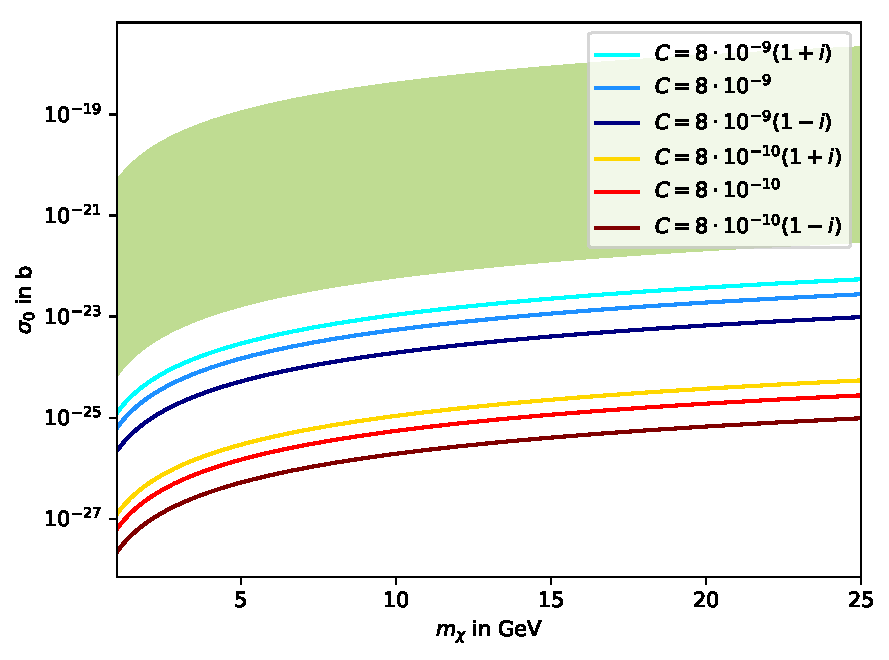
\includegraphics[width=.87\textwidth]{Bilder/Allgemein11.pdf}
\end{frame}
%\begin{frame}[noframenumbering]{Einschränkung aus den $B$-Zerfällen 1}
%\framesubtitle{Real- und Imaginärteil von $C$ variabel}
%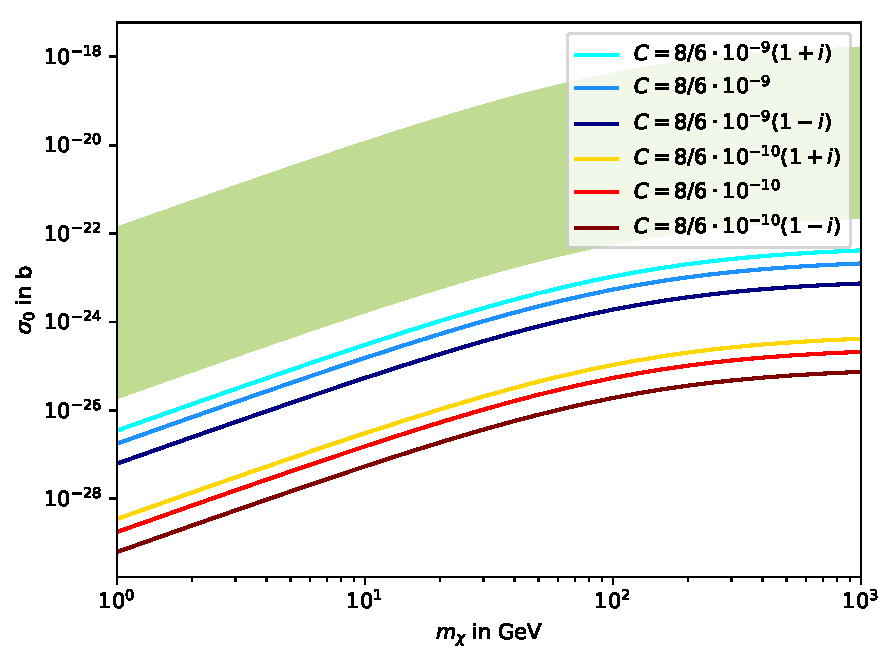
\includegraphics[width=\textwidth]{Bilder/Allgemein116.pdf}
%\end{frame}


\begin{frame}{Einschränkung aus den $B$-Zerfällen 2}
\framesubtitle{$\SI{540}{\giga\electronvolt}\lessapprox\sfrac{m_{Z'}}{g'}\lessapprox\SI{4.9}{\tera\electronvolt}$, $\text{Re}(C) = \SI{8e-10}{\giga\electronvolt}^{-2}$, $\text{Im}(C)$ variabel}
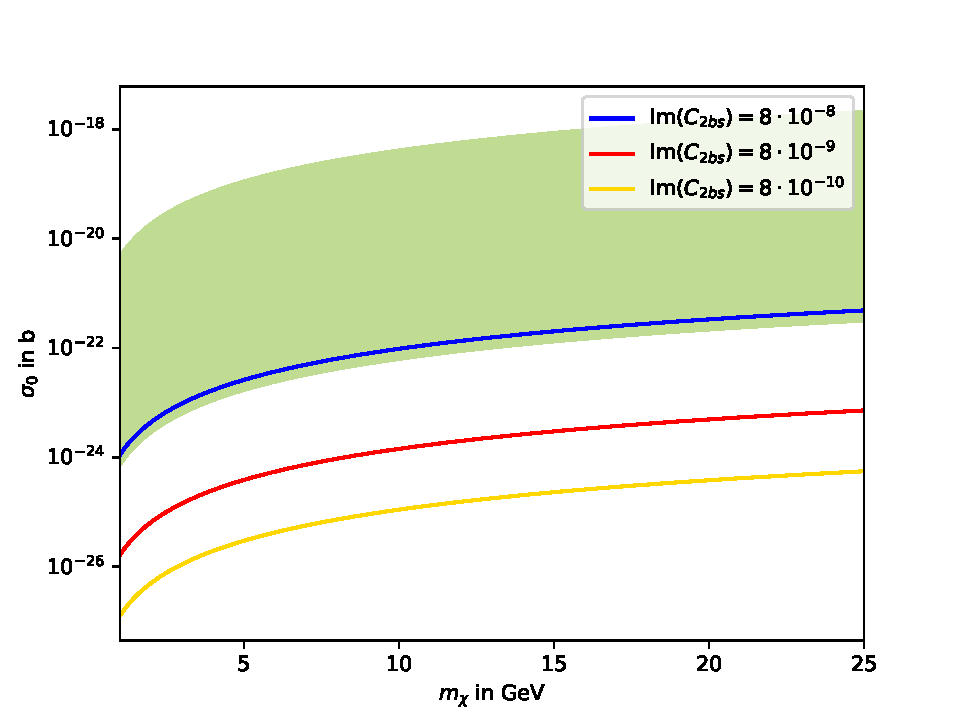
\includegraphics[width=.87\textwidth]{Bilder/Im11.pdf}
\end{frame}
%\begin{frame}[noframenumbering]{Einschränkung aus den $B$-Zerfällen 2}
%\framesubtitle{Fester Realteil, variabler Imaginärteil}
%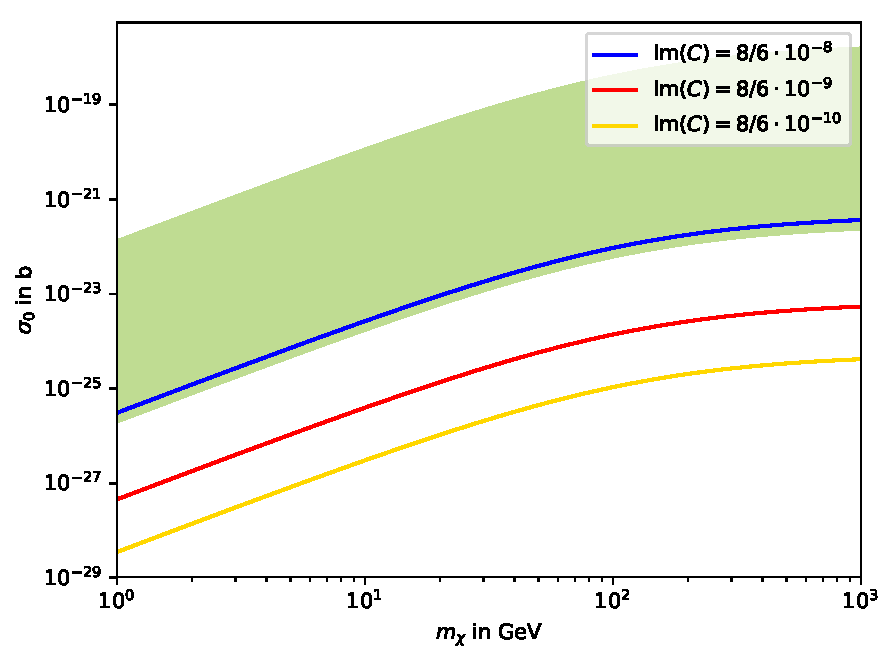
\includegraphics[width=\textwidth]{Bilder/Im116.pdf}
%\end{frame}


\begin{frame}{Einschränkung aus der Relic Density und Direct Detection}
\framesubtitle{$m_{Z'} \approx 2m_\chi$, $g'=\SI{2e-3}{}$}
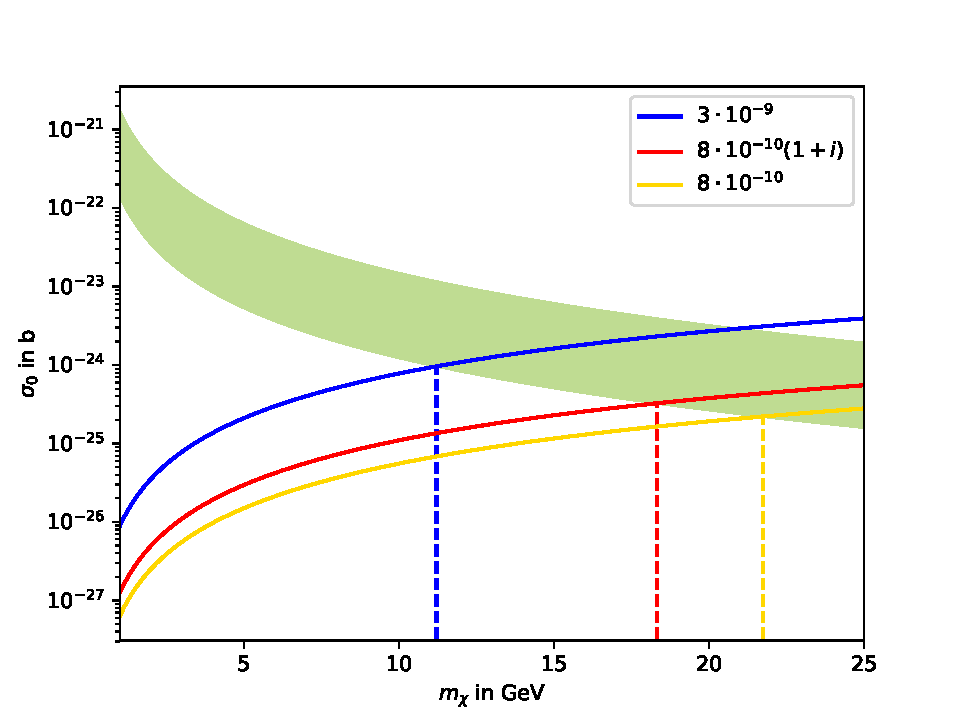
\includegraphics[width=.87\textwidth]{Bilder/Relic11.pdf}
\end{frame}
%\begin{frame}[noframenumbering]{Einschränkung aus der Relic Density}
%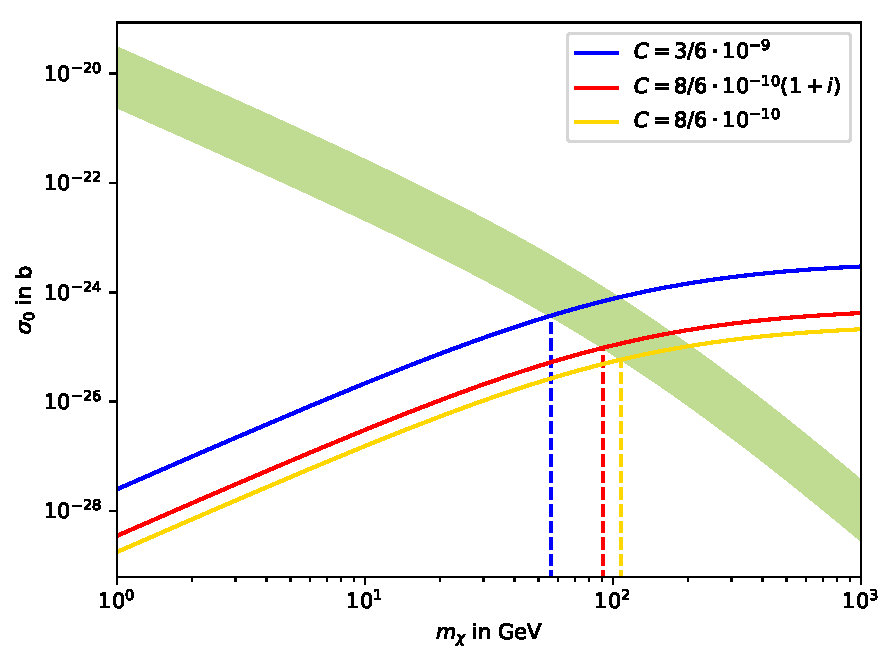
\includegraphics[width=\textwidth]{Bilder/Relic116.pdf}
%\end{frame}